\documentclass[tikz]{standalone}

\usetikzlibrary{arrows}
\usetikzlibrary{arrows.meta}

\begin{document}

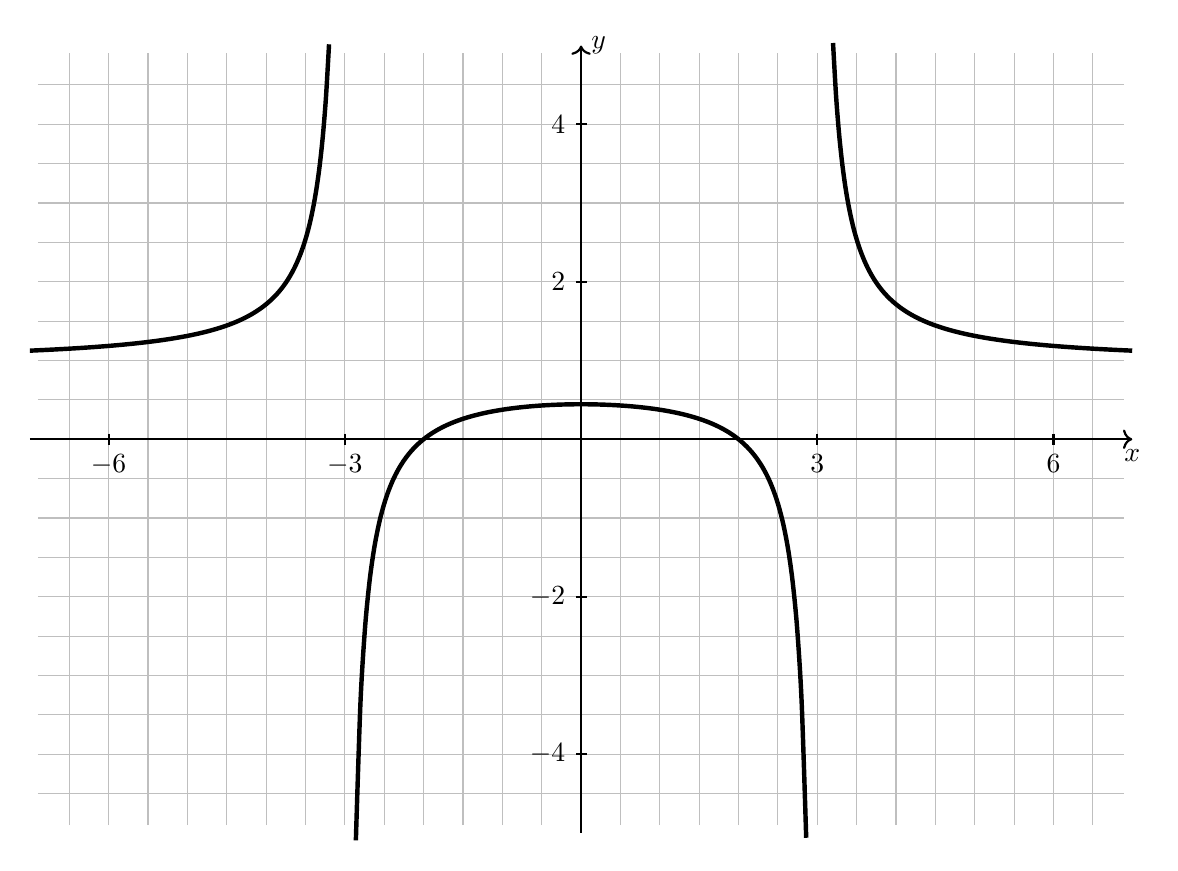
\begin{tikzpicture}[baseline=70,ultra thick,smooth,domain=-7:7,variable=\x,scale=1]

    % create a white background, with a black frame
    % \draw [fill=white] (-7.25,-3.25) rectangle (7.25,5.25); 
    
    % draw a grid
    \draw[step=5.0mm, lightgray, thin] (-6.9,-4.9) grid (6.9,4.9); 
    %\draw[step=1cm, gray] (-6.9,-2.9) grid (6.9,4.9); 
    
    
    % draw axes
    \draw [->,thick] (-7,0) -- (7,0) node[below] {$x$}; 
    \draw [->,thick] (0,-5) -- (0,5) node[right] {$y$};
    
    % tick marks
    \foreach \x in {-6,-3,3,6} 
        \draw [thick] (\x cm,2pt) -- (\x cm,-2pt) node[below] {$\x$};
    \foreach \y in {-4, -2,2,4} 
        \draw [thick] (2pt,\y cm) -- (-2pt,\y cm) node[left] {$\y$};
    
    \draw plot [domain=-7:-3.2, samples=100] (\x,{(\x*\x - 4) / (\x*\x - 9)}); 
    \draw plot [domain=-2.86:2.86, samples=100] (\x,{(\x*\x - 4) / (\x*\x - 9)}); 
    \draw plot [domain=3.2:7, samples=100] (\x,{(\x*\x - 4) / (\x*\x - 9)}); 

\end{tikzpicture}

\end{document} 